\chapter{Capa de Estrategia}
\section{Introducción}

Esta capa plantea los aspectos estratégicos de la empresa. Cada uno de los puntos de vista que contiene esta capa presenta una perspectiva diferente sobre el modelado de la dirección estratégica de alto nivel y la composición de la organización\cite{ArchiMate3.0.1}. 

Esta capa  busca establecer y conocer los diferentes planes estratégicos que van a tomar lugar en los procesos de negocio actuales de la organización, por lo tanto, es importante tener en cuenta los conceptos utilizados en la capa de Motivación para así facilitar la identificación de los diferentes usos e interacciones que se presentan con esta capa. Para una adecuada apropiación de la conceptualización de esta capa, se implementa el uso de cuatro diferentes puntos de vista: Estrategia, Mapa de capacidad,Realización de Resultado y Mapa de recurso.

A continuación se presentan cada uno de los puntos de vista de la capa de Estrategia  a partir del soporte realizado por el Área de Investigación de Análisis de datos a los investigadores de la Subdirección de Investigaciones, otras Subdirecciones y demás unidades funcionales del Instituto de Cancerología.

%-------------Punto de Vista Estretegia----------%
\newpage
\section{Punto de Vista de la Estrategia}

El punto de vista de la estrategia permite a la organización modelar una visión general estratégica de alto nivel de los cursos de acción de la empresa, las capacidades y recursos que los respaldan, y los resultados previstos\cite{ArchiMate3.0.1}. 

En la Figura \ref{PvEstretegia} se plantea el Caso para el Punto de Vista de la Estrategia con cada uno de los elementos que interactúan entre sí. 

\begin{figure}[h!]
	\centering
	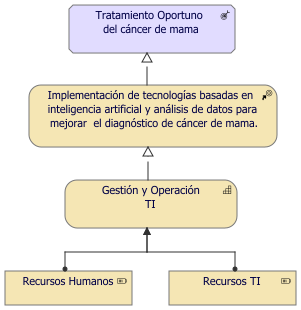
\includegraphics[width=0.75\linewidth]{ARQUITECTURA/imgs/CapaEstrategica/1_PvEstrategia}
	\caption{Punto de Vista de la Estrategia}
	\label{PvEstretegia}
\end{figure}

\begin{enumerate}[label=\textbf{\arabic*})]
	
\item  \textbf{Tratamiento Oportuno del cáncer de mama:} Hace referencia al \textit{resultado} que espera obtener el Instituto de Cancerología a través del Área de Investigación de Análisis de datos. Este resultado esta basado en la rapidez y veracidad de los diagnósticos de cáncer de mama generados para cada paciente que tiene como consecuencia un tratamiento a tiempo que permita sanar dicho cáncer.

\item  \textbf{Implementación de tecnologías basadas en  inteligencia artificial y análisis de datos para 	mejorar  el diagnóstico de cáncer de mama :} Hace referencia al \textit{curso de acción} planteado por el Instituto de Cancerología a través del Área de Investigación de Análisis de datos para obtener un \textit{Tratamiento Oportuno del cáncer de mama}.

\item  \textbf{Gestión y Operación TI:} Hace referencia a la \textit{capacidad} con respecto a la gestión y operación de Tecnologías de la Informacion del Área de Investigación de Análisis de datos para realizar el curso de acción de \textit{Implementación de tecnologías basadas en  inteligencia artificial y análisis de datos para 	mejorar  el diagnóstico de cáncer de mama}. Esta asignado a los siguientes recursos:

\begin{itemize}
	\item  \textbf{\textit{Recursos Humanos:}} Este recurso hace referencia a los coordinadores, lideres técnicos,Especialistas en Oncología, científicos de datos  y desarrolladores del Área de Investigación de Análisis de datos los cuales poseen habilidades en la gestión y operación de las Tecnologías de la Informacion.
	
	\item  \textbf{\textit{Recursos TI:}} Este recurso hace referencia a las herramientas basadas en las Tecnologías de la Informacion que influyen en la realización de diagnósticos oncológicos. En este caso la principal herramienta para la generación de diagnósticos de cáncer de mama es la aplicación web \textit{BreastApp}.
\end{itemize}
	
 \end{enumerate}

%-------------Punto de Vista Capa de Capacidad----------%
\newpage
\section{Punto de Vista del Mapa de Capacidad}

El punto de vista del mapa de capacidad permite crear una visión general estructurada de las capacidades de la empresa. Un mapa de capacidades generalmente muestra dos o tres niveles de las capacidades en toda la organización. Puede, por ejemplo, usarse como un mapa de calor para identificar áreas de inversión. En algunos casos, un mapa de capacidades también puede mostrar resultados específicos entregados por estas capacidades\cite{ArchiMate3.0.1}. 

En la Figura \ref{PvMapaCapacidad} se plantea el Caso para el Punto de Vista del Mapa de Capacidad con cada uno de los elementos que interactúan entre sí. 

\begin{figure}[h!]
	\centering
	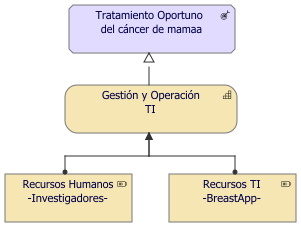
\includegraphics[width=0.75\linewidth]{ARQUITECTURA/imgs/CapaEstrategica/2_PvMapaCapacidad}
	\caption{Punto de Vista del Mapa de Capacidad}
	\label{PvMapaCapacidad}
\end{figure}

\begin{enumerate}[label=\textbf{\arabic*})]
	
\item  \textbf{Tratamiento Oportuno del cáncer de mama:} Hace referencia al \textit{resultado} que espera obtener el Instituto de Cancerología a través del Área de Investigación de Análisis de datos. Este resultado esta basado en la rapidez y veracidad de los diagnósticos de cáncer de mama generados para cada paciente que tiene como consecuencia un tratamiento a tiempo que permita sanar dicho cáncer.

\newpage
\item  \textbf{Gestión y Operación TI:} Hace referencia a la \textit{capacidad} con respecto a la gestión y operación de Tecnologías de  la Informacion del Área de Investigación de Análisis de datos para realizar el curso de acción de \textit{Implementación de tecnologías basadas en  inteligencia artificial y análisis de datos para 	mejorar  el diagnóstico de cáncer de mama}. Esta asignado a los siguientes recursos:
	
	\begin{itemize}
		\item  \textbf{\textit{Recursos Humanos:}} Este recurso hace referencia a los coordinadores, lideres técnicos,Especialistas en Oncología, científicos de datos  y desarrolladores del Área de Investigación de Análisis de datos los cuales poseen habilidades en la gestión y operación de las Tecnologías de la Informacion.
		
		\item  \textbf{\textit{Recursos TI:}} Este recurso hace referencia a las herramientas basadas en las Tecnologías de la Informacion que influyen en la realización de diagnósticos oncológicos. En este caso la principal herramienta para la generación de diagnósticos de cáncer de mama es la aplicación web \textit{BreastApp}.
	\end{itemize}
	
\end{enumerate}

%-------------Punto de Vista Capa de Capacidad----------%
\newpage
\section{Punto de Vista de la Realización de Resultado}

El punto de vista de realización del resultado se utiliza para mostrar los resultados orientados al negocio ,considerados de alto nivel, son realizados por las capacidades y los elementos centrales de la organización\cite{ArchiMate3.0.1}. 

En la Figura \ref{PvRealizacion} se plantea el Caso para el Punto de Vista de la realización de resultado con cada uno de los elementos que interactúan entre sí. 

\begin{figure}[h!]
	\centering
	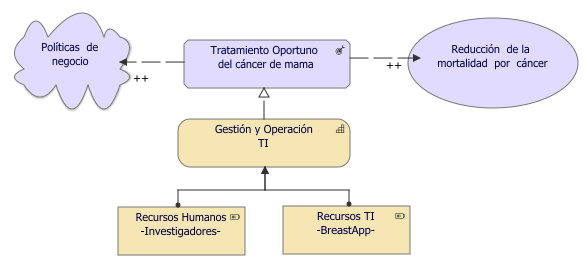
\includegraphics[width=1\linewidth]{ARQUITECTURA/imgs/CapaEstrategica/3_PvRealizacion}
	\caption{Punto de Vista de la Realización de Resultado}
	\label{PvRealizacion}
\end{figure}


\begin{enumerate}[label=\textbf{\arabic*})]
	
\item  \textbf{Tratamiento Oportuno del cáncer de mama:} Hace referencia al \textit{resultado} que espera obtener el Instituto de Cancerología a través del Área de Investigación de Análisis de datos. Este resultado esta basado en la rapidez y veracidad de los diagnósticos de cáncer de mama generados para cada paciente que tiene como consecuencia un tratamiento a tiempo que permita sanar dicho cáncer.

\item  \textbf{Políticas de negocio:} Hace referencia al elemento asociado al core del instituto de Cancerología el cual esta basado en el control integral del cáncer a través de la atención y el cuidado de pacientes, la investigación, la formación de talento humano y el desarrollo de acciones en salud pública. Se puede observar que  el  \textit{Tratamiento Oportuno del cáncer de mama} obtenido como resultado  de la estrategia planteada por el  Área de Investigación de Análisis de datos tiene un efecto positivo en las políticas de negocio.

\newpage
\item  \textbf{Reducción  de la mortalidad  por cáncer:} Hace referencia a el valor   del core de la visión del instituto de Cancerología fundamentado en la reducción de la mortalidad por cáncer, sobre la base de la innovación y la tecnología. Se puede observar que  el  \textit{Tratamiento Oportuno del cáncer de mama} obtenido como resultado  de la estrategia planteada por el  Área de Investigación de Análisis de datos de datos tiene un efecto positivo en este valor de la organización.

\item  \textbf{Gestión y Operación TI:} Hace referencia a la \textit{capacidad} con respecto a la gestión y operación de Tecnologías de  la Informacion del Área de Investigación de Análisis de datos para realizar el curso de acción de \textit{Implementación de tecnologías basadas en  inteligencia artificial y análisis de datos para 	mejorar  el diagnóstico de cáncer de mama}. Esta asignado a los siguientes recursos:
	
\begin{itemize}
		\item  \textbf{\textit{Recursos Humanos:}} Este recurso hace referencia a los coordinadores, lideres técnicos,Especialistas en Oncología, científicos de datos  y desarrolladores del Área de Investigación de Análisis de datos los cuales poseen habilidades en la gestión y operación de las Tecnologías de la Informacion.
		
		\item  \textbf{\textit{Recursos TI:}} Este recurso hace referencia a las herramientas basadas en las Tecnologías de la Informacion que influyen en la realización de diagnósticos oncológicos. En este caso la principal herramienta para la generación de diagnósticos de cáncer de mama es la aplicación web \textit{BreastApp}.
\end{itemize}
	
\end{enumerate}


%-------------Punto de Vista Capa de Capacidad----------%
\newpage
\section{Punto de Vista de Mapa de Recurso}

El punto de vista de mapa de recurso permite tener una visión general estructurada de los recursos de la organización describiendo las  relaciones entre los recursos y las capacidades a las que están asignados \cite{ArchiMate3.0.1}. 

En la Figura \ref{PvMapaRecurso} se plantea el Caso para el Punto de Vista de Mapa de Recurso con cada uno de los elementos que interactúan entre sí. 

\begin{figure}[h!]
	\centering
	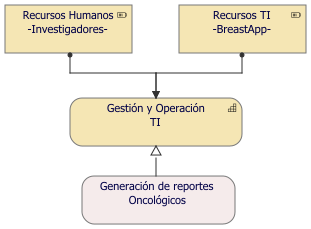
\includegraphics[width=0.77\linewidth]{ARQUITECTURA/imgs/CapaEstrategica/4_PvMapaRecurso}
	\caption{Punto de Vista de Mapa de Recurso}
	\label{PvMapaRecurso}
\end{figure}

\begin{enumerate}[label=\textbf{\arabic*})]
	

\item  \textbf{Gestión y Operación TI:} Hace referencia a la \textit{capacidad} con respecto a la gestión y operación de Tecnologías de  la Informacion del Área de Investigación de Análisis de datos para realizar el curso de acción de \textit{Implementación de tecnologías basadas en  inteligencia artificial y análisis de datos para 	mejorar  el diagnóstico de cáncer de mama}. Esta asignado a los siguientes recursos:
	
	\begin{itemize}
		\item  \textbf{\textit{Recursos Humanos:}} Este recurso hace referencia a los coordinadores, lideres técnicos,Especialistas en Oncología, científicos de datos  y desarrolladores del Área de Investigación de Análisis de datos los cuales poseen habilidades en la gestión y operación de las Tecnologías de la Informacion.
		\item  \textbf{\textit{Recursos TI:}} Este recurso hace referencia a las herramientas basadas en las Tecnologías de la Informacion que influyen en la realización de diagnósticos oncológicos. En este caso la principal herramienta para la generación de diagnósticos de cáncer de mama es la aplicación web \textit{BreastApp}.
	\end{itemize}

\item  \textbf{Generación de reportes oncológicos:} Es el paquete de trabajo principal del instituto de Cancerología basado en la estrategia planteada y los recursos disponibles identificados. La meta es construir una  aplicación web que genere  informes tipo reporte con base a los resultados arrojados por  diferentes modelos de Machine Learning, en donde se de un resultado definitivo acerca del  padecimiento de Cáncer de mama.Este diagnostico se realiza con el propósito de dar soporte a los investigadores de la Subdirección de Investigaciones, otras Subdirecciones y demás unidades funcionales del Instituto  de Cancerología.
	
\end{enumerate}













